%%%%%%%%%%%%%%%%%%%%%%%%%%%%%%%%%%%%%%%%%%%%%%%
%%%     Declarations (skip to Begin Document, line 112, for parts you fill in)
%%%%%%%%%%%%%%%%%%%%%%%%%%%%%%%%%%%%%%%%%%%%%%%

\documentclass[10pt]{article}

\usepackage{geometry}  % Lots of layout options.  See http://en.wikibooks.org/wiki/LaTeX/Page_Layout
\geometry{letterpaper}  % ... or a4paper or a5paper or ... 
\usepackage{fullpage}  % somewhat standardized smaller margins (around an inch)
\usepackage{setspace}  % control line spacing in latex documents
\usepackage[parfill]{parskip}  % Activate to begin paragraphs with an empty line rather than an indent

\usepackage{amsmath,amssymb}  % latex math
\usepackage{empheq} % http://www.ctan.org/pkg/empheq
\usepackage{bm,upgreek}  % allows you to write bold greek letters (upper & lower case)

% for typsetting algorithm pseudocode see http://en.wikibooks.org/wiki/LaTeX/Algorithms_and_Pseudocode
\usepackage{algorithmic,algorithm}  

\usepackage{graphicx}  % inclusion of graphics; see: http://en.wikibooks.org/wiki/LaTeX/Importing_Graphics
% allow easy inclusion of .tif, .png graphics
\DeclareGraphicsRule{.tif}{png}{.png}{`convert #1 `dirname #1`/`basename #1 .tif`.png}

\usepackage{color}  % http://en.wikibooks.org/wiki/LaTeX/Colors

\long\def\ans#1{{\color{blue}{\em #1}}}
\long\def\ansnem#1{{\color{blue}#1}}
\long\def\boldred#1{{\color{red}{\bf #1}}}

% Useful package for syntax highlighting of specific code (such as python) -- see below
\usepackage{listings}  % http://en.wikibooks.org/wiki/LaTeX/Packages/Listings
\usepackage{textcomp}

%%% The following lines set up using the listings package
\renewcommand{\lstlistlistingname}{Code Listings}
\renewcommand{\lstlistingname}{Code Listing}

%%% Specific for python listings
\definecolor{gray}{gray}{0.5}
\definecolor{green}{rgb}{0,0.5,0}

\lstnewenvironment{python}[1][]{
\lstset{
language=python,
basicstyle=\footnotesize,  % could also use this -- a little larger \ttfamily\small\setstretch{1},
stringstyle=\color{red},
showstringspaces=false,
alsoletter={1234567890},
otherkeywords={\ , \}, \{},
keywordstyle=\color{blue},
emph={access,and,break,class,continue,def,del,elif ,else,%
except,exec,finally,for,from,global,if,import,in,i s,%
lambda,not,or,pass,print,raise,return,try,while},
emphstyle=\color{black}\bfseries,
emph={[2]True, False, None, self},
emphstyle=[2]\color{green},
emph={[3]from, import, as},
emphstyle=[3]\color{blue},
upquote=true,
morecomment=[s]{"""}{"""},
commentstyle=\color{gray}\slshape,
emph={[4]1, 2, 3, 4, 5, 6, 7, 8, 9, 0},
emphstyle=[4]\color{blue},
literate=*{:}{{\textcolor{blue}:}}{1}%
{=}{{\textcolor{blue}=}}{1}%
{-}{{\textcolor{blue}-}}{1}%
{+}{{\textcolor{blue}+}}{1}%
{*}{{\textcolor{blue}*}}{1}%
{!}{{\textcolor{blue}!}}{1}%
{(}{{\textcolor{blue}(}}{1}%
{)}{{\textcolor{blue})}}{1}%
{[}{{\textcolor{blue}[}}{1}%
{]}{{\textcolor{blue}]}}{1}%
{<}{{\textcolor{blue}<}}{1}%
{>}{{\textcolor{blue}>}}{1},%
%framexleftmargin=1mm, framextopmargin=1mm, frame=shadowbox, rulesepcolor=\color{blue},#1
framexleftmargin=1mm, framextopmargin=1mm, frame=single,#1
}}{}
%%% End python code listing definitions

%%% Specific for matlab listings
\definecolor{dkgreen}{rgb}{0,0.6,0}
\definecolor{gray}{rgb}{0.5,0.5,0.5}
\definecolor{mauve}{rgb}{0.58,0,0.82}
 
\lstnewenvironment{matlab}[1][]{
\lstset{ %
  language=Matlab,                % the language of the code
  basicstyle=\footnotesize,           % the size of the fonts that are used for the code
  numbers=left,                   % where to put the line-numbers
  numberstyle=\tiny\color{gray},  % the style that is used for the line-numbers
  stepnumber=2,                   % the step between two line-numbers. If it's 1, each line 
                                  % will be numbered
  numbersep=5pt,                  % how far the line-numbers are from the code
  backgroundcolor=\color{white},      % choose the background color. You must add \usepackage{color}
  showspaces=false,               % show spaces adding particular underscores
  showstringspaces=false,         % underline spaces within strings
  showtabs=false,                 % show tabs within strings adding particular underscores
  frame=single,                   % adds a frame around the code
  rulecolor=\color{black},        % if not set, the frame-color may be changed on line-breaks within not-black text (e.g. commens (green here))
  tabsize=2,                      % sets default tabsize to 2 spaces
  captionpos=t,                   % sets the caption-position to top
  breaklines=true,                % sets automatic line breaking
  breakatwhitespace=false,        % sets if automatic breaks should only happen at whitespace
  title=\lstname,                   % show the filename of files included with \lstinputlisting;
                                  % also try caption instead of title
  keywordstyle=\color{blue},          % keyword style
  commentstyle=\color{dkgreen},       % comment style
  stringstyle=\color{mauve},         % string literal style
  escapeinside={\%*}{*)},            % if you want to add LaTeX within your code
  morekeywords={*,...}               % if you want to add more keywords to the set
  framexleftmargin=1mm, framextopmargin=1mm, frame=single,#1 % display caption
} }{}
%%% End matlab code listing definitions

%%%%%%%%%%%%%%%%%%%%%%%%%%%%%%%%%%%%%%%%%%%%%%%
%%%     Begin Document
%%%%%%%%%%%%%%%%%%%%%%%%%%%%%%%%%%%%%%%%%%%%%%%

\begin{document}

\begin{center}
    {\Large {\bf ISTA 421/521 -- Homework 1}} \\
    % {\Large {\bf \ans{Answers}}} \\
    Due: Friday, September 5, 5pm (to the class D2L dropbox) \\
    8 points total
\end{center}

\begin{flushright}
Emanuel Carlos de Alcantara Valente  %% Fill in your name here

Undergraduate %% select which you are!
\end{flushright}

\vspace{1cm}
All written portions of the homework must be submitted to the D2L dropbox as a .pdf.

In the following, FCMA refers to the course text: Simon Rogers and Mark Girolami (2012), {\em A First Course in Machine Learning}.  (All questions from the book are reproduced here in full, so you do not need the book to proceed.)

For general notes on using latex to typeset math, see: {\tt http://en.wikibooks.org/wiki/LaTeX/Mathematics}
\vspace{.5cm}

%%%%%%%%%%%%%%%%
%%%     Problems
%%%%%%%%%%%%%%%%

\begin{enumerate}

%%%     Problem 1
\item[1.]
{\bf Exercise 1.1} from FCMA p.35 [0.5 pts]

\begin{figure}[htb]
\begin{center}
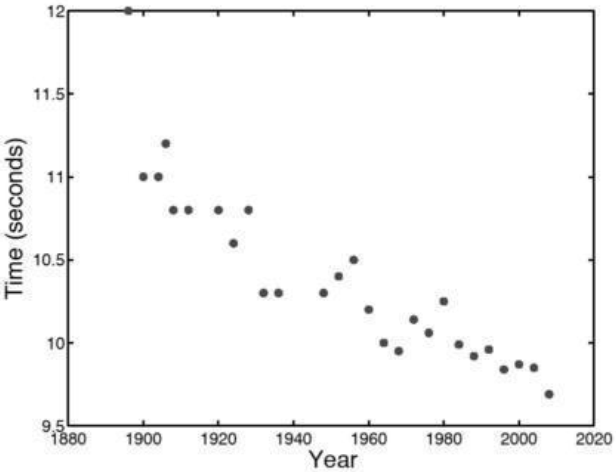
\includegraphics[width=6cm]{figs/figure1-1_p2.png}
\caption{Reproduction of figure 1.1, Olympic men's 100m data}
\end{center}
\end{figure}
By examining Figure 1.1 [from p. 2 of FCMA, reproduced here], estimate (by hand / in your head) the kind of values we should expect for $w_0$ and $w_1$ (e.g., High? Low?  Positive?  Negative?).

{\bf Solution.} We expect that $w_0$ will be high and positive. Through the figure, we can infer that in order to have a good model (in this case it is a linear function) it should have an intercept (where the line intercepts the t-axis in $x = 0$) high ( $\sim > 11$) and positive. 

The $w_1$ is expected to be negative and low. Through the same way, a good model will have a negative gradient because the line is descending ( at least $100^{\circ} < slope(line) < 170^{\circ}$). Therefore, the tangent of this angle will be negative and low.


%%% $<$Solution goes here.$>$


\end{enumerate}

\newpage
%%% Note for next three problems:
NOTE: The following three exercises (2, 3, and 4) review basic linear algebra concepts; we will review these briefly in Lecture 3.  
\begin{enumerate}

\item[] Notation conventions:
\begin{itemize}
\item Script variables, such as $x_{n2}$ and $w_1$ represent scalar values
\item Lowercase bold-face variables, such as $\mathbf{x}_n$ and $\mathbf{w}$, represent vectors
\item Uppercase bold-face variables, such as $\mathbf{X}$, represent $n$ (rows) $\times ~m$ (columns) matrices
\item Note that because all indexes in the following are either a value between 0, 1, ..., 9, or a scalar, $n$, I am representing multiple dimension indexes without a comma, as it is unambiguous; e.g., $x_{32}$ is the element scalar value of $\mathbf{X}$ at row 3, column 2.  When we have to refer to specific index values greater than 9, we'll use commas, such as $x_{32,3}$ is the scalar value in the 32nd row and 3rd column.
\item `$\top$' in expressions like $\mathbf{w}^\top$ indicates the transpose operator.
\end{itemize}

%%%     Problem 2
\item[2.]
{\bf Exercise 1.3} from FCMA p.35  [1pt]

Show that:
\begin{eqnarray*}
\mathbf{w}^\top\mathbf{X}^\top\mathbf{X}\mathbf{w} = w_0^2 \left( \sum_{n=1}^N x_{n1}^2 \right) + 2w_0w_1 \left( \sum_{n=1}^N x_{n1}x_{n2} \right) + w_1^2 \left( \sum_{n=1}^N x_{n2}^2 \right),
\end{eqnarray*}
where
\begin{eqnarray*}
\mathbf{w} = 
    \begin{bmatrix}
    w_0 \\[0.3em]
    w_1
    \end{bmatrix}
    ,
\mathbf{X} = 
    \begin{bmatrix}
    x_{11} & x_{12} \\[0.3em]
    x_{21} & x_{22} \\[0.3em]
    x_{31} & x_{32} \\[0.3em]
    \vdots & \vdots \\[0.3em]
    x_{N1} & x_{N2}
    \end{bmatrix}
    .
\end{eqnarray*}
(Hint -- it's probably easiest to do the $\mathbf{X}^\top\mathbf{X}$ first!)

{\bf Solution.} Let's solve first  $\mathbf{X}^\top\mathbf{X}$

$\mathbf{X}^\top\mathbf{X} = $ 
\begin{bmatrix}
    x_{11} & x_{21} & x_{31} & \hdots  & x_{N1}\\[0.1em]
    x_{12} & x_{22} & \x_{32} & \hdots & x_{N2}\\[0.1em]
    \end{bmatrix}
 \begin{bmatrix}
    x_{11} & x_{12} \\[0.3em]
    x_{21} & x_{22} \\[0.3em]
    x_{31} & x_{32} \\[0.3em]
    \vdots & \vdots \\[0.3em]
    x_{N1} & x_{N2}
    \end{bmatrix} =
    
=\begin{bmatrix}
x_{11}x_{11} + x_{21}x_{21} + \hdots + x_{N1}x_{N1} & x_{11}x_{12} + x_{21}x_{22} + \hdots + x_{N1}x_{N2}\\[0.1em]
x_{12}x_{11} + x_{22}x_{21} + \hdots + x_{N2}x_{N1} & x_{12}x_{12} + x_{22}x_{22} + \hdots + x_{N2}x_{N2}\\[0.1em]
\end{bmatrix} = 
\begin{bmatrix}
\sum_{n=1}^N x_{n1}^2 &  \sum_{n=1}^N x_{n1}x_{n2}\\[0.3em]
\sum_{n=1}^N x_{n1}x_{n2} &  \sum_{n=1}^N x_{n2}^2\\[0.3em]
\end{bmatrix}

    
Now, we will calculate: $\mathbf{w}^\top\mathbf{X}^\top\mathbf{X}$

 $\mathbf{w}^\top\mathbf{X}^\top\mathbf{X} = $  
 \begin{bmatrix}
w_{0} & w_{1}
\end{bmatrix}
\begin{bmatrix}
\sum_{n=1}^N x_{n1}^2 &  \sum_{n=1}^N x_{n1}x_{n2}\\[0.3em]
\sum_{n=1}^N x_{n1}x_{n2} &  \sum_{n=1}^N x_{n2}^2\\[0.3em]
\end{bmatrix} = 

=\begin{bmatrix}
w_{0}\sum_{n=1}^N x_{n1}^2 + w_{1}\sum_{n=1}^N x_{n1}x_{n2} & w_{0}\sum_{n=1}^N x_{n1}x_{n2} + w_{1}\sum_{n=1}^N x_{n2}^2\\[0.3em]
\end{bmatrix}

Finally:

$\mathbf{w}^\top\mathbf{X}^\top\mathbf{X}\mathbf{w} = $ 
\begin{bmatrix}
w_{0}\sum_{n=1}^N x_{n1}^2 + w_{1}\sum_{n=1}^N x_{n1}x_{n2} & w_{0}\sum_{n=1}^N x_{n1}x_{n2} + w_{1}\sum_{n=1}^N x_{n2}^2\\[0.3em]
\end{bmatrix}
\begin{bmatrix}
w_{0} \\ 
w_{1}
\end{bmatrix} =

=\begin{bmatrix}
w_{0}^{2}\sum_{n=1}^N x_{n1}^2 + w_{0}w_{1}\sum_{n=1}^N x_{n1}x_{n2} + w_{0}w{1}\sum_{n=1}^N x_{n1}x_{n2} + w_{1}^{2}\sum_{n=1}^N x_{n2}^2\\[0.3em]
\end{bmatrix} = 

= w_0^2 \left( \sum_{n=1}^N x_{n1}^2 \right) + 2w_0w_1 \left( \sum_{n=1}^N x_{n1}x_{n2} \right) + w_1^2 \left( \sum_{n=1}^N x_{n2}^2 \right) \\[1.0cm]



%%%     Problem 3
\item[3.]
{\bf Exercise 1.4} from FCMA p.35  [1pt]

Using $\mathbf{w}$ and $\mathbf{X}$ as defined in the previous exercise, show that ${(\mathbf{X}\mathbf{w})}^\top = {\mathbf{w}}^\top{\mathbf{X}}^\top$ by multiplying out both sides.

{\bf Solution.}

Multiplying the left side:

${(\mathbf{X}\mathbf{w})}^\top =  \left( \begin{bmatrix}
    x_{11} & x_{12} \\[0.3em]
    x_{21} & x_{22} \\[0.3em]
    x_{31} & x_{32} \\[0.3em]
    \vdots & \vdots \\[0.3em]
    x_{n1} & x_{n2}
    \end{bmatrix}
    \begin{bmatrix}
    w_0 \\[0.3em]
    w_1
    \end{bmatrix} \right)^\top = 
    \left( \begin{bmatrix}
    x_{11}w_{0} + x_{12}w_{1} \\[0.3em]
    x_{21}w_{0} + x_{22}w_{1} \\[0.3em]
    x_{31}w_{0} + x_{32}w_{1} \\[0.3em]
    \vdots  \\[0.3em]
    x_{n1}w_{0} + x_{n2}w_{1}
    \end{bmatrix}
    \right)^\top = 
    \begin{bmatrix}
    w_{0}x_{11} + w_{1}x_{12} &  w_{0}x_{21} + w_{1}x_{22} & \hdots &   w_{0}x_{n1} + w_{1}x_{n2}  
    \end{bmatrix}   
   $
   

Multiplying the right side:

${\mathbf{w}}^\top{\mathbf{X}}^\top = 
\begin{bmatrix}
w_{0} & w_{1}
\end{bmatrix} 
\begin{bmatrix}
x_{11} & x_{21} & \hdots  & x_{N1}\\[0.1em]
x_{12} & x_{22} & \hdots & x_{N2}\\[0.1em]
\end{bmatrix}
=
 \begin{bmatrix}
    w_{0}x_{11} + w_{1}x_{12} &  w_{0}x_{21} + w_{1}x_{22} & \hdots &   w_{0}x_{n1} + w_{1}x_{n2}  
    \end{bmatrix}   


$

Therefore, ${(\mathbf{X}\mathbf{w})}^\top = {\mathbf{w}}^\top{\mathbf{X}}^\top$.


%%%     Problem 4
\item[4.]
{\bf Exercise 1.5} from FCMA p.35  [1pt]

When multiplying a scalar by a vector (or matrix), we multiply each element of the vector (or matrix) by that scalar.  For $\mathbf{x}_n = {[ x_{n1}, x_{n2} ]}^\top$, $\mathbf{t} = {[ t_1,...,t_N ]}^\top$, $\mathbf{w} = {[ w_0, w_1 ]}^\top$, and
\begin{eqnarray*}
\mathbf{X} = 
    \begin{bmatrix}
    {\mathbf{x}_{1}}^\top \\[0.3em]
    {\mathbf{x}_{2}}^\top \\[0.3em]
    \vdots \\[0.3em]
    {\mathbf{x}_{N}}^\top
    \end{bmatrix}
\end{eqnarray*}
show that
\begin{eqnarray*}
\sum_{n} \mathbf{x}_n t_n = \mathbf{X}^\top\mathbf{t}
\end{eqnarray*}
and
\begin{eqnarray*}
\sum_{n} \mathbf{x}_n \mathbf{x}_n ^\top \mathbf{w} = \mathbf{X}^\top\mathbf{X} \mathbf{w}
\end{eqnarray*}

{\bf Solution.} 

We will show that $\sum_{n} \mathbf{x}_n t_n = \mathbf{X}^\top\mathbf{t}$

Developing the left side:

$\sum_{n} \mathbf{x}_n t_n = \mathbf{x}_1 t_1 + \mathbf{x}_2 t_2 + \hdots + \mathbf{x}_n t_n =
\begin{bmatrix}
x_{11} t_1 \\
x_{12} t_1 
\end{bmatrix} 
+
\begin{bmatrix}
x_{21} t_2 \\
x_{22} t_2 
\end{bmatrix} 
+
\hdots
+
\begin{bmatrix}
x_{n1} t_n \\
x_{n2} t_n 
\end{bmatrix} 
=
\begin{bmatrix}
x_{11} t_1 + x_{11} t_2 + \hdots + x_{n1} t_n  \\
x_{12} t_1 + x_{22} t_2 + \hdots + x_{n2} t_n  \\
\end{bmatrix} 
=

=\begin{bmatrix}
\sum_{n} {x}_{n1} t_n  \\[0.3em]
\sum_{n} {x}_{n2} t_n 
\end{bmatrix} 
$ \\[1.0cm]

Developing the right side:

$\mathbf{X}^\top\mathbf{t} 
=
\begin{bmatrix}
    x_{11} & x_{21}  & \hdots  & x_{n1}\\[0.1em]
    x_{12} & x_{22}  & \hdots & x_{n2}\\[0.1em]
    \end{bmatrix}
 \begin{bmatrix}
    t_1 \\[0.1em]
    t_2 \\[0.1em]
    \vdots \\[0.1em]
    t_n \\[0.1em]
    \end{bmatrix}
=
= \begin{bmatrix}
x_{11} t_1 + x_{11} t_2 + \hdots + x_{n1} t_n  \\
x_{12} t_1 + x_{22} t_2 + \hdots + x_{n2} t_n  \\
\end{bmatrix} 
=
\begin{bmatrix}
\sum_{n} {x}_{n1} t_n  \\[0.3em]
\sum_{n} {x}_{n2} t_n 
\end{bmatrix} 
$

Therefore, $\sum_{n} \mathbf{x}_n t_n = \mathbf{X}^\top\mathbf{t}$.\\[1.cm]

Now, we will show that $\sum_{n} \mathbf{x}_n \mathbf{x}_n ^\top \mathbf{w} = \mathbf{X}^\top\mathbf{X} \mathbf{w}$

Starting by the left side, we will have:

$\sum_{n} \mathbf{x}_n \mathbf{x}_n ^\top \mathbf{w}=
\sum_{n}\left(
\begin{bmatrix}
{x}_{n1}  \\[0.3em]
{x}_{n2}
\end{bmatrix}
\begin{bmatrix}
{x}_{n1}  & {x}_{n2}
\end{bmatrix}
\begin{bmatrix}
{w}_{0}  \\[0.3em]
{w}_{1}
\end{bmatrix}
\right)
=
\sum_{n}
\begin{bmatrix}
{x}_{n1}^2  & {x}_{n1}{x}_{n2}\\[0.3em]
{x}_{n1}{x}_{n2} & {x}_{n2}^2
\end{bmatrix}
\begin{bmatrix}
{w}_{0}  \\[0.3em]
{w}_{1}
\end{bmatrix}
=
\sum_{n}
\begin{bmatrix}
{w}_{0}{x}_{n1}^2  + {w}_{1}{x}_{n1}{x}_{n2}\\[0.3em]
{w}_{0}{x}_{n1}{x}_{n2} +  {w}_{1}{x}_{n2}^2
\end{bmatrix}
$ \\[1.0 cm]

On the other hand, the right side will be:

$\mathbf{X}^\top\mathbf{X} \mathbf{w}$

We have seen in the Exercise \textbf{1.3} that: $\mathbf{X}^\top\mathbf{X} = 
\begin{bmatrix}
\sum_{n=1}^N x_{n1}^2 &  \sum_{n=1}^N x_{n1}x_{n2}\\[0.3em]
\sum_{n=1}^N x_{n1}x_{n2} &  \sum_{n=1}^N x_{n2}^2\\[0.3em]
\end{bmatrix}
$

So, $\mathbf{X}^\top\mathbf{X} \mathbf{w} = 
\begin{bmatrix}
\sum_{n=1}^N x_{n1}^2 &  \sum_{n=1}^N x_{n1}x_{n2}\\[0.3em]
\sum_{n=1}^N x_{n1}x_{n2} &  \sum_{n=1}^N x_{n2}^2\\[0.3em]
\end{bmatrix}
\begin{bmatrix}
{w}_{0}\\[0.3em]
{w}_{1}
\end{bmatrix}
=
\begin{bmatrix}
{w}_{0}\sum_{n=1}^N x_{n1}^2 +  {w}_{1}\sum_{n=1}^N x_{n1}x_{n2}\\[0.3em]
{w}_{0}\sum_{n=1}^N x_{n1}x_{n2} +  {w}_{1}\sum_{n=1}^N x_{n2}^2\\[0.3em]
\end{bmatrix}
=

=\begin{bmatrix}
\sum_{n=1}^N {w}_{0}x_{n1}^2 +  \sum_{n=1}^N {w}_{1}x_{n1}x_{n2}\\[0.3em]
\sum_{n=1}^N {w}_{0}x_{n1}x_{n2} +  \sum_{n=1}^N {w}_{1}x_{n2}^2\\[0.3em]
\end{bmatrix}
=
\sum_{n}
\begin{bmatrix}
{w}_{0}{x}_{n1}^2  + {w}_{1}{x}_{n1}{x}_{n2}\\[0.3em]
{w}_{0}{x}_{n1}{x}_{n2} +  {w}_{1}{x}_{n2}^2
\end{bmatrix}

$

Therefore, $\sum_{n} \mathbf{x}_n \mathbf{x}_n ^\top \mathbf{w} = \mathbf{X}^\top\mathbf{X} \mathbf{w}$



\newpage
%%%     Problem 5
\item[5.] 
{\bf Plotting Exercise} -- three parts

\begin{itemize}
\item[{\bf A.}] [0.5pt] Use the provided python script {\tt plotlinear.py} and plot three lines (parameters of your choosing).  This requires you have you python environment set up.  Place the output graphic in your pdf submission and provide a descriptive caption that indicates the intercept and slope values you used to generate the lines.  (\LaTeX~users can use the commented code in the HW latex template for inserting the figure.)

{\bf Solution.} 

\begin{figure}[htb]
\begin{center}
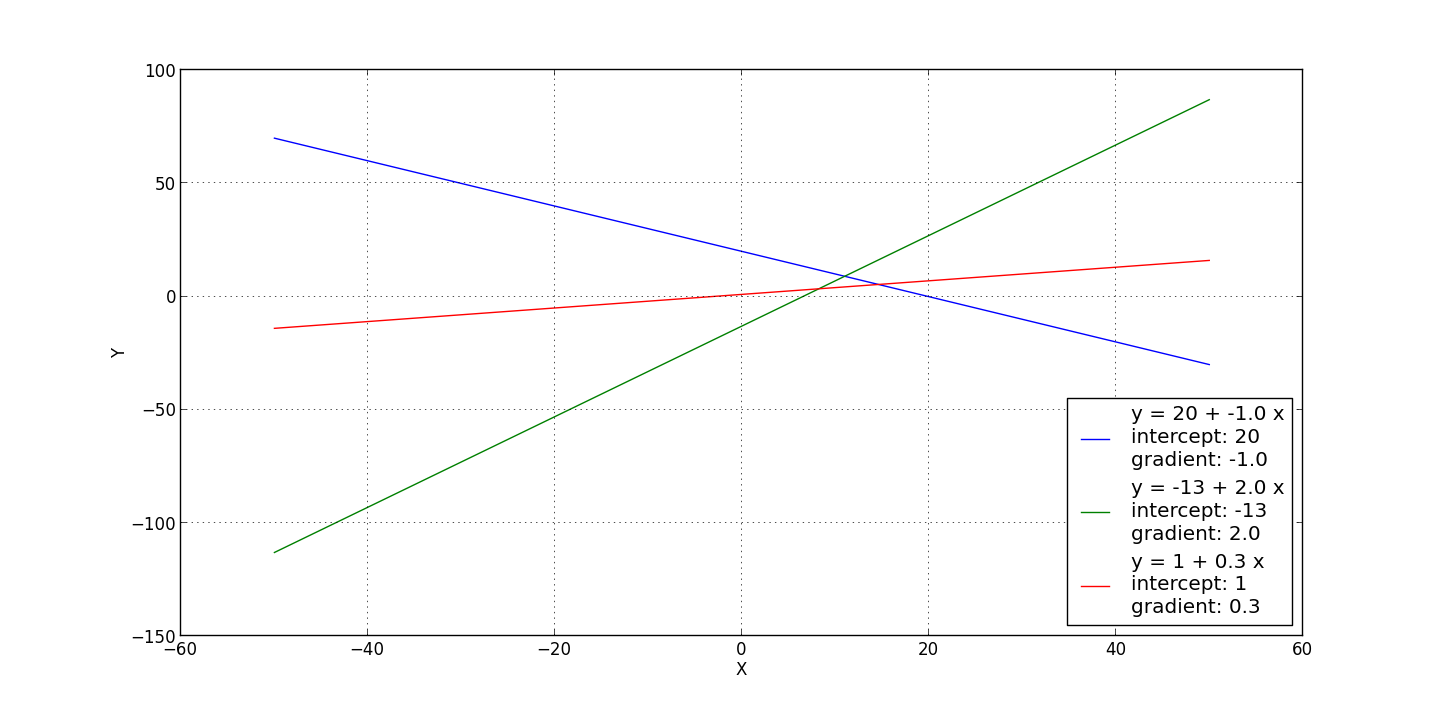
\includegraphics[width=14cm]{figs/figure_q5-a.png} %% enter path to your figure
\caption{Solution}
\end{center}
\end{figure}

\item[{\bf B.}] [0.5pt] Now, try another plot: generate a vector whose entries are the values of $\sin(\mathbf{x})$ for $\mathbf{x}$ in the range $[0,10]$ in steps of $0.01$, and plot it.  Label the y-axis `sin(x)', the x-axis 'x values' and provide a title for the plot, `Sine Function for x from 0.0 to 10.0'.  Include your plot in the pdf submission.

{\bf Solution.}
\begin{figure}[htb]
\begin{center}
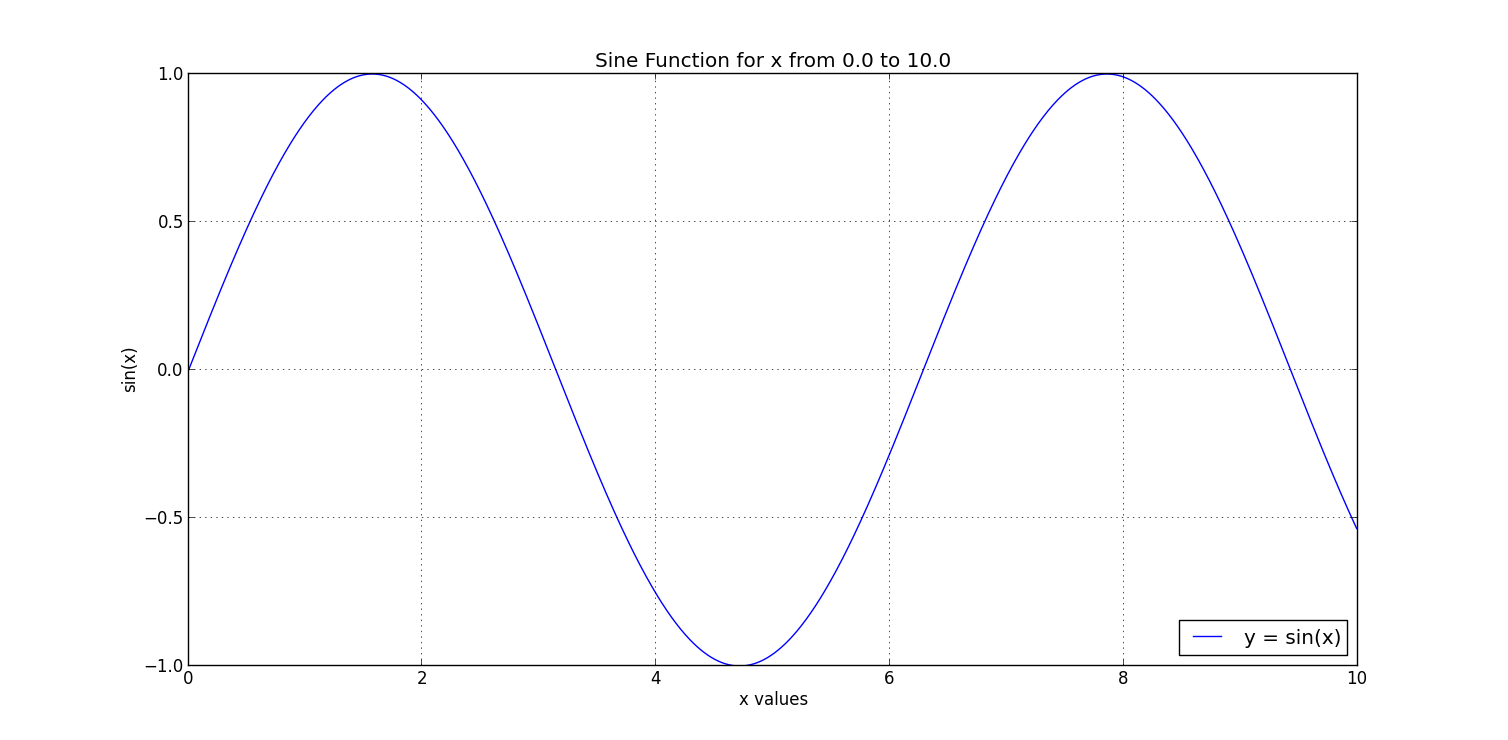
\includegraphics[width=14cm]{figs/sinx.png}
\caption{$\sin(\mathbf{x})$ for $\mathbf{x}$ in range $[0,10]$ in steps of $0.01$}
\end{center}
\end{figure}


\newpage

\item[{\bf C.}] [0.5pt] Finally, put your script code in the pdf file.  

For \LaTeX~users: you can use the following python code listing environment.  The code currently listed here is from the {\tt plotlinear.py} script; replace the code there with the code you wrote for generating the $\sin$ function.

{\bf Solution.}

%%% Begin python code output
\begin{python}[caption={ {\tt plot-sin.py} script}, label=Sine Function for x from 0.0 to 10.0]
## plot-sin.py
import numpy as np
import matplotlib.pyplot as plt

plt.ion()

#x-axis: from 0.0 to 10.0 (steps: 0.01)
x = np.arange(0, 10, 0.01);

#plt.figure(0)

#Define x and y labels as well as title
plt.xlabel("x values")
plt.ylabel("sin(x)")
plt.title("Sine Function for x from 0.0 to 10.0 ")
#our grid (just for a better reading)
plt.grid()

#Ploting our function and its label
plt.plot(x, np.sin(x), label="y = sin(x)")
#loc = 4 bottom right
plt.legend(loc=4)

#holds our graph on screen
raw_input("\nPress <ENTER> to exit...");


\end{python}
%%% End python code output

\end{itemize}

 

\newpage
%%%     Problem 6
\item[6.] 
{\bf More Programming in Python Practice}

\begin{itemize}
\item[{\bf A.}]  [1pt]
Write a short script that initializes the random number generator
\begin{itemize}
\item[] python: {\tt numpy.random.seed(seed=1)}
\end{itemize}
Followed by creating two three-dimensional column vectors using
\begin{itemize}
\item[] python: {\tt random.rand} (used in the context of code to generate the vectors)
\end{itemize}
Represent the random variables as $\mathbf{a}$ and $\mathbf{b}$ (be sure you issue the call to set the random seed immediately before creating these variables).  Print them at the terminal and copy-and-paste the result here. (If using \LaTeX, use the {\tt verbatim} environment to display).

{\bf Solution.}

\begin{verbatim}

[emanuel@localhost code]$ python hw1-6a.py 
a = [  4.17022005e-01   7.20324493e-01   1.14374817e-04]
b = [ 0.30233257  0.14675589  0.09233859]

\end{verbatim}

\item[{\bf B.}]  [2pts]
Using the values of $\mathbf{a}$ and $\mathbf{b}$, compute the following and display the result two ways: (1) copy-and-paste the output (from the python interpreter/terminal; again, in \LaTeX~use the {\tt verbatim} environment), (2) typeset the output (e.g., using the \LaTeX~math environment).
\begin{enumerate}
\item[1.] $\mathbf{a} + \mathbf{b} = ~?$

Solution:

\begin{verbatim}
[emanuel@localhost code]$ python hw1-6b1.py 
a = [  4.17022005e-01   7.20324493e-01   1.14374817e-04]
b = [ 0.30233257  0.14675589  0.09233859]
a + b = [ 0.71935458  0.86708038  0.09245297]
\end{verbatim} \\[5.5 cm]

Soluton in \hologo{LaTeX}:

$\mathbf{a} + \mathbf{b} = 
\begin{bmatrix}
4.17022005e*10^{-1} \\
7.20324493*10^{-1} \\
1.14374817*10^{-4}
\end{bmatrix}
+
\begin{bmatrix}
0.30233257 \\
0.14675589 \\
0.09233859
\end{bmatrix}
=
\begin{bmatrix}
0.71935458 \\
0.86708038 \\
0.09245297
\end{bmatrix}


$


\item[2.] $\mathbf{a} \circ \mathbf{b} = ~?$  (element-wise multiply; Note: the notation $\mathbf{a} \circ \mathbf{b}$ is also known as the Hadamard product, the entrywise product, or the Schur product.)

Solution:

\begin{verbatim}
[emanuel@localhost code]$ python hw1-6b2.py 
a = [  4.17022005e-01   7.20324493e-01   1.14374817e-04]
b = [ 0.30233257  0.14675589  0.09233859]
a * b = [  1.26079336e-01   1.05711863e-01   1.05612099e-05]
\end{verbatim} \\ [5.0 cm]

Solution in \hologo{LaTeX}:

$\mathbf{a} \circ \mathbf{b} = 
\begin{bmatrix}
4.17022005e*10^{-1} \\
7.20324493*10^{-1} \\
1.14374817*10^{-4}
\end{bmatrix}
\circ
\begin{bmatrix}
0.30233257 \\
0.14675589 \\
0.09233859
\end{bmatrix}
=
\begin{bmatrix}
 1.26079336*10^{-1} \\
1.05711863*10^{-1} \\
1.05612099*10^{-5}
\end{bmatrix}


$

\item[3.] $\mathbf{a}^\top \mathbf{b} = ~?$  (also called the dot-product)


{\bf Solution.}

\begin{verbatim}
[emanuel@localhost code]$ python hw1-6b3.py 
a = [  4.17022005e-01   7.20324493e-01   1.14374817e-04]
b = [ 0.30233257  0.14675589  0.09233859]
aT.b = 0.231801759448
\end{verbatim}


Solution in \hologo{LaTeX}:

$\mathbf{a}^\top \mathbf{b} =
\begin{bmatrix}
4.17022005e*10^{-1} \\
7.20324493*10^{-1} \\
1.14374817*10^{-4}
\end{bmatrix}
^\top
\begin{bmatrix}
0.30233257 \\
0.14675589 \\
0.09233859
\end{bmatrix}
=

=\begin{bmatrix}
4.17022005e*10^{-1} & 7.20324493*10^{-1} & 1.14374817*10^{-4}
\end{bmatrix}
\begin{bmatrix}
0.30233257 \\
0.14675589 \\
0.09233859
\end{bmatrix}
=
0.231801759448


$

%%\end{enumerate}


Now, set the random seed to 2 and immediately generate a random $3 \times 3$ matrix $\mathbf{X}$.  In your solution, display the value of $\mathbf{X}$.  Using $\mathbf{X}$ and the earlier values of $a$ and $b$, compute the following in python and typeset the results in two ways, as before.

\begin{verbatim}
[emanuel@localhost code]$ python hw1-6b4.py 
X = 
[[ 0.4359949   0.02592623  0.54966248]
 [ 0.43532239  0.4203678   0.33033482]
 [ 0.20464863  0.61927097  0.29965467]]
\end{verbatim}


Solution in \hologo{LaTeX}:

$\mathbf{X}
=
\begin{bmatrix}
0.4359949 & 0.02592623 &  0.54966248 \\
0.43532239 & 0.4203678  & 0.33033482 \\
0.20464863 & 0.61927097  & 0.29965467 \\
\end{bmatrix}

$


\item[4.] $\mathbf{a}^\top\mathbf{X} = ~?$

{\bf Solution.}


\begin{verbatim}
[emanuel@localhost code]$ python hw1-6b4.py 
aT.X = [ 0.49541626  0.31368386  0.46720388]

\end{verbatim}


Solution in \hologo{LaTeX}:

$\mathbf{a}^\top\mathbf{X}
=
\begin{bmatrix}
4.17022005e*10^{-1} & 7.20324493*10^{-1} & 1.14374817*10^{-4}
\end{bmatrix}
\begin{bmatrix}
0.4359949 & 0.02592623 &  0.54966248 \\
0.43532239 & 0.4203678  & 0.33033482 \\
0.20464863 & 0.61927097  & 0.29965467 \\
\end{bmatrix}
=

=\begin{bmatrix}
 0.49541626 & 0.31368386 & 0.46720388
\end{bmatrix}
$


\item[5.] $\mathbf{a}^\top\mathbf{X}\mathbf{b} = ~?$

{\bf Solution.}

\begin{verbatim}
[emanuel@localhost code]$ python hw1-6b5.py 
aT.X.b = 
0.238956376181
\end{verbatim}

Solution in \hologo{LaTeX}:

$\mathbf{a}^\top\mathbf{X}\mathbf{b} = 
(\mathbf{a}^\top\mathbf{X})\mathbf{b} = 
\begin{bmatrix}
 0.49541626 & 0.31368386 & 0.46720388
\end{bmatrix}
\begin{bmatrix}
0.30233257 \\
0.14675589 \\
0.09233859
\end{bmatrix}
=
0.238956376181

$


\item[6.] $\mathbf{X}^{-1} = ~?$
\end{enumerate}

\end{itemize}
{\bf Solution.} 

\begin{verbatim}
[emanuel@localhost code]$ python hw1-6b6.py 
X^-1 = 
[[-1.20936675  5.11771977 -3.42333228]
 [-0.96691719  0.279414    1.46561347]
 [ 2.82418088 -4.07257903  2.64627411]]
 \end{verbatim}

Solution in \hologo{LaTeX}:

$\mathbf{X}^{-1} =
\begin{bmatrix}
0.4359949 & 0.02592623 &  0.54966248 \\
0.43532239 & 0.4203678  & 0.33033482 \\
0.20464863 & 0.61927097  & 0.29965467 \\
\end{bmatrix}^{-1}
= 
\begin{bmatrix}
-1.20936675 & 5.11771977 & -3.42333228 \\
-0.96691719  & 0.279414    & 1.46561347 \\
2.82418088 & -4.07257903 & 2.64627411 \\
\end{bmatrix}

$


\end{enumerate}

\end{document}
